\documentclass[10pt,twocolumn,letterpaper]{article}

% Những thứ riêng của tôi
\usepackage{booktabs}
% \usepackage{caption}
% \captionsetup[table]{skip=8pt}   % Chỉ ảnh hưởng tới bảng
\usepackage{stfloats}  % Thêm dòng này vào phần tiền đề
\usepackage{float}
\usepackage[T5]{fontenc}

% \usepackage{fontspec}
\usepackage[english]{babel}

% load Lao via babelprovide, turn on "onchar=ids" for automatic shaping
\babelprovide[import,onchar=ids fonts]{vietnamese}

% main (rm) font for Latin
\babelfont{rm}{Noto Serif}

% Lao text in Noto Serif Lao at 1.2× scale
\babelfont[vietnamese]{rm}{Noto Serif}
\babelfont[vietnamese]{sf}{Noto Serif}

% alternate (sans-serif) font for Latin
\babelfont{alt}{Lato}

% Lao text in Noto Serif Lao for the alt family too
\babelfont[vietnamese]{alt}{Noto Serif}

\usepackage{cvpr}
\usepackage{times}
\usepackage{epsfig}
\usepackage{graphicx}
\usepackage{amsmath}
\usepackage{amssymb}

% \makeatletter
% \def\cvprsubsection{\@startsection {subsection}{2}{\z@}
%     {8pt plus 2pt minus 2pt}{6pt}{\bfseries\normalsize}}
% \makeatother

% Bao gồm các gói khác ở đây, trước hyperref.

% Nếu bạn bình luận hyperref rồi bỏ bình luận lại, bạn nên xóa
% egpaper.aux trước khi chạy lại latex.  (Hoặc chỉ cần nhấn 'q' vào lần chạy latex đầu tiên,
% để nó hoàn thành, và bạn sẽ rõ ràng).
\usepackage[breaklinks=true,bookmarks=false]{hyperref}

\cvprfinalcopy % *** Bỏ chú thích dòng này cho bài nộp cuối cùng

\def\cvprPaperID{****} % *** Nhập CVPR Paper ID tại đây
\def\httilde{\mbox{\tt\raisebox{-.5ex}{\symbol{126}}}}

% For some reason \renewtablename wasnt working so I had to add this hack
\usepackage{caption}
\captionsetup[table]{name=Bảng}
% \renewcommand{\tablename}{Bảng}
\renewcommand{\figurename}{Hình}   % or whatever you like instead of "Hình"

% This makes the font slightly bigger than base (10) and bold in Subsection headings rather than using ptmb
% after those:
\addto\captionsenglish{%
  \renewcommand{\figurename}{Hình}%
}

\makeatletter
\def\abstract{%
  \centerline{\large\bf Tóm tắt}% <-- your new label
  \vspace*{12pt}%
  \it%
}
\makeatother

\makeatletter
\def\cvprsubsection{%
  \@startsection{subsection}{2}{\z@}%
    {8pt plus 2pt minus 2pt}{6pt}%
    % {\normalfont\bfseries\selectfont}%
    {\normalfont\bfseries\fontsize{11}{13}\selectfont}%
}
\makeatother

% So this hardcodes the style for the numbers in the section/subsection headings so they're bold
\font\elvbf=ptmb scaled 1100
\font\elvbfs=ptmb scaled 1200
\makeatletter
% Section number: Large + bold
\renewcommand\thesection{%
  {\elvbfs\arabic{section}}%
}

% Subsection number: normalsize + bold + custom punctuation
\renewcommand\thesubsection{%
  {\elvbf
   \arabic{section}.\arabic{subsection}}%
}
\makeatother

% Các trang được đánh số trong chế độ gửi bài, và không đánh số trong bản camera-ready
%\ifcvprfinal\pagestyle{empty}\fi
\setcounter{page}{1}
\begin{document}

%%%%%%%%% TIÊU ĐỀ
\title{Tài liệu hướng dẫn dựa trên dữ liệu về ECDO - Phần 1/2: Hiểu biết hiện tại về Lý thuyết “Trái Đất lật” ECDO — Hiệu ứng Dzhanibekov do quá trình tách rời tỏa nhiệt giữa lớp lõi và lớp manti của Trái Đất}

\author{Junho\\
Xuất bản tháng 2 năm 2025\\
Trang web (Tải tài liệu tại đây): \href{https://sovrynn.github.io}{sovrynn.github.io}\\
Kho nghiên cứu ECDO: \href{https://github.com/sovrynn/ecdo}{github.com/sovrynn/ecdo}\\
{\tt\small junhobtc@proton.me}
% Đối với một bài báo mà tất cả các tác giả đều ở cùng một tổ chức,
% hãy bỏ qua các dòng sau cho đến dấu ``}'' kết thúc.
% Các tác giả và địa chỉ bổ sung có thể được thêm vào với ``\and'',
% giống như tác giả thứ hai.
% Để tiết kiệm không gian, chỉ sử dụng địa chỉ email hoặc trang chủ, không sử dụng cả hai
% \and
% xxx
% Institution2\\
% Dòng đầu tiên của địa chỉ institution2\\
% {\tt\small secondauthor@i2.org}
}

\maketitle
%\thispagestyle{empty}

%%%%%%%%% TÓM TẮT
\begin{abstract}
Tháng 5 năm 2024, một tác giả ẩn danh trên mạng có bút danh là “The Ethical Skeptic” \cite{0} đã chia sẻ một lý thuyết đột phá có tên là Hiệu ứng Dzhanibekov do quá trình tách rời tỏa nhiệt giữa lớp lõi và lớp manti của Trái Đất (ECDO — Exothermic Core-Mantle Decoupling Dzhanibekov Oscillation) \cite{1}. Lý thuyết này cho rằng Trái Đất từng trải qua những thay đổi đột ngột và thảm khốc trong trục quay, dẫn đến các trận đại hồng thủy toàn cầu khi đại dương, do quán tính quay, tràn vào lục địa. Ngoài ra, lý thuyết còn trình bày các quá trình địa vật lý liên quan, kèm theo dữ liệu cho thấy lần "Trái Đất lật" tiếp theo có thể sắp xảy ra. Mặc dù các dự đoán về lũ lụt thảm họa và ngày tận thế không phải là điều mới, nhưng lý thuyết ECDO lại đặc biệt có tính thuyết phục nhờ cách tiếp cận mang tính khoa học, hiện đại, đa ngành và dựa trên dữ liệu.

Bài viết này là phần đầu tiên trong bản tóm lược gồm hai phần của 6 tháng nghiên cứu độc lập \cite{2,20} về lý thuyết ECDO. Bài viết nhấn mạnh ba điểm chính:

\begin{flushleft}
\begin{enumerate}
    \item Một sự kiện "Trái Đất lật" tương tự ECDO đã xảy ra nhiều lần trong lịch sử gần đây của loài người, được chứng minh qua các truyền thuyết về trận đại hồng thuỷ và các dấu hiệu địa chất về lũ lụt diện rộng ở các lục địa.
    \item Có thể xác định được hướng và biên độ xấp xỉ của các lần Trái Đất lật trong quá khứ.
    \item Các dữ liệu về từ trường Trái Đất và địa vật lý gần đây cho thấy rằng có thể sắp xảy ra lần lật Trái Đất tiếp theo, và biến đổi khí hậu có thể là do những thay đổi sâu bên trong Trái Đất chứ không phải do con người.
\end{enumerate}
\end{flushleft}

Ngoài ra, tôi cũng trình bày các cơ chế vật lý gây ra hiện tượng “Trái Đất lật” mà lý thuyết ECDO đề xuất.

Trong bài viết này, tôi giữ quan điểm khách quan bằng cách tập trung vào dữ liệu thực nghiệm, tránh các phần hấp dẫn nhưng còn mang tính suy đoán của lý thuyết, và nhấn mạnh rằng đây là chủ đề mà nhân loại cần cấp thiết nghiên cứu thêm.
\end{abstract}

%%%%%%%%% BODY TEXT
\section{Giới thiệu}

Các câu chuyện về trận đại hồng thuỷ không phải là điều mới — thực tế, chúng xuất hiện trong mọi nền văn hoá lớn trên toàn cầu, trải dài qua mọi cái nôi của nền văn minh. Biểu đồ minh hoạ (Hình \ref{fig:1}) từ bản tổng hợp 267 câu chuyện về lũ lụt \cite{3} cho thấy hầu như tất cả khu vực có người sinh sống trên Trái Đất đều có những câu chuyện về lũ lụt.

% \begin{figure}[h]
% \begin{figure}[b]
\begin{figure}[h]
\begin{center}
% \fbox{\rule{0pt}{2in} \rule{0.9\linewidth}{0pt}}
   \includegraphics[width=1\linewidth]{b.png}
\end{center}
   \caption{Vị trí các câu chuyện về lũ lụt trên khắp thế giới \cite{3}.}
\label{fig:1}
\label{fig:onecol}
\end{figure}

Khi xem xét kỹ hơn những câu chuyện này, ta thấy đây không phải những trận lũ thông thường mà là các thảm họa mang tính hủy diệt kèm theo các lũ lụt đã quét sạch các lục địa.

\subsection{Những câu chuyện về thảm họa của người bản địa châu Mỹ}

Các câu chuyện của người bản địa châu Mỹ ghi lại một số mô tả sống động nhất về những thảm họa lớn của Trái Đất. Người Hopi, một bộ tộc người bản địa châu Mỹ sống ở đông bắc Arizona, kể rằng, \textit{"..Sótuknang đã kêu gọi Người Kiến mở cánh cửa dẫn vào thế giới dưới lòng đất cho những người được chọn. Khi họ đã an toàn dưới lòng đất, Sótuknang ra lệnh cho cặp song sinh Pöqánghoya và Palöngawhoya rời khỏi vị trí canh giữ ở hai đầu bắc và nam của trục thế giới, nơi họ được giao nhiệm vụ giữ cho Trái Đất quay đúng cách. \textbf{Cặp song sinh vừa rời khỏi vị trí thì thế giới, không còn ai kiểm soát, trở nên mất cân bằng, quay cuồng điên đảo, rồi lộn vòng hai lần.} Các ngọn núi lao xuống biển với những tiếng va đập dữ dội, biển và hồ nước tràn lên đất liền; và khi thế giới quay trong không gian lạnh giá và không sự sống, nó đã đóng băng thành băng đá rắn"} \cite{4}.

Nhiều câu chuyện này mô tả chính xác quy mô khổng lồ của trận đại hồng thủy, kể lại rằng nước biển đã dâng cao nhấn chìm tất cả trừ những đỉnh núi cao nhất. Người Skokomish, sống ở bang Washington, kể rằng, \textit{"Đấng Linh Thiêng Vĩ Đại tức giận trước sự độc ác của con người và muông thú nên đã quyết định xóa sạch mọi sinh vật ở Trái Đất, chỉ giữ lại những con vật tốt, một người đàn ông tốt và gia đình ông. Theo chỉ dẫn của Đấng Linh Thiêng Vĩ Đại, người đàn ông bắn một mũi tên lên đám mây, rồi bắn tiếp một mũi tên khác vào mũi tên trước đó, cứ tiếp tục như vậy, tạo thành một sợi dây bằng mũi tên nối từ mây xuống mặt đất. Những con vật tốt và người tốt trèo lên. Các con vật xấu và rắn cũng cố trèo lên, nhưng người đàn ông đã bẻ gãy sợi dây mũi tên đó. \textbf{Sau đó, Đấng Linh Thiêng Vĩ Đại tạo ra nhiều ngày mưa, lũ lụt dâng lên đến tận ranh giới tuyết trên Takhoma (núi Ranier).} Sau khi tất cả người xấu và con vật xấu bị nhấn chìm, Đấng Linh Thiêng Vĩ Đại dừng mưa, nước dần rút xuống, rồi người tốt và các con vật tốt trèo xuống"} \cite{3}. Để tham khảo, núi Rainier là một núi lửa đang hoạt động ở Washington có độ cao 4392,5 m so với mực nước biển.

Câu chuyện về trận lụt của người Makah ở bang Washington đặc biệt đề cập đến một trận lụt nhiều giai đoạn có dòng nước "rất ấm", cho thấy đây không phải là trận lụt thông thường: \textit{"Biển dâng cao đến mức cắt đứt mũi đất. Rồi nước biển rút xuống mức thấp nhất sau bốn ngày, để lại Vịnh Neah khô ráo. Rồi biển lại dâng lên, nhấn chìm tất cả trừ các đỉnh núi. \textbf{Nước dâng lên rất ấm.} Những người có xuồng chất đầy đồ đạc và bị trôi dạt xa về phía bắc. Nhiều người chết khi xuồng bị mắc vào cây. Bốn ngày sau, biển trở lại bình thường, và mọi người nhận ra mình đã trôi dạt xa về phía bắc, nơi con cháu của họ vẫn còn sống đến nay"} \cite{3}.

\subsection{Những câu chuyện đại nạn của Trung Hoa}

Ở phía bên kia Thái Bình Dương, nền văn minh Trung Hoa hiện đại được cho là bắt đầu từ một trận đại hồng thuỷ. Triều đại Hạ, được cho là tồn tại vào khoảng năm 2000 TCN, được Đại Vũ lập nên. Ông là người đã chế ngự trận Đại hồng thủy của Cống và Vu \cite{6}. Thời ông, \textit{"... phép lạ được cho là đã xảy ra khi mặt trời suốt mười ngày không lặn, rừng núi bốc cháy và vô vàn loài côn trùng ghê tởm xuất hiện... Một con sóng khổng lồ “chạm tới trời” đổ ập xuống đất Trung Hoa. \textbf{"Nước dâng cao tới tận các ngọn núi, không thể nhìn thấy chân núi đâu nữa"}... "Sức hủy diệt của nước lũ là không thể tưởng tượng nổi", hoàng đế nói. "Trong làn nước mênh mông khổng lồ ấy, chúng ôm trọn cả đồi núi và vượt qua những đỉnh cao vĩ đại, đe dọa trời bằng nước lũ." Hoàng đế ra lệnh phải tìm mọi cách mở đường cho nước thoát ra khỏi các thung lũng giữa núi. Trong nhiều năm, dân chúng vất vả làm việc, cố gắng khai thông đồng bằng và thung lũng bị ngập bằng cách đào kênh và thoát nước cho đồng ruộng. Trong thời gian dài, mọi nỗ lực đều vô ích. Vị đại thần chịu trách nhiệm cho công việc to lớn và cấp bách này là Khwan đã bị xử tử vì thất bại... và chỉ có con trai ông là Vũ mới thành công trong việc dẫn nước lũ thoát ra ngoài. Thành tựu ấy được đánh giá rất cao nên Vũ đã trở thành hoàng đế Trung Hoa sau vua Thuấn, người kế vị đầu tiên của Nghiêu"} \cite{5}.

Dường như không chỉ có Trung Hoa bị lụt, mà thậm chí còn phải đo lại các hướng chính và chuyển động của mặt trời và mặt trăng, cho thấy có thể Trái Đất đã thay đổi chuyển động quay trong trận lụt: \textit{\textbf{"Vị hoàng đế này đã cử các học giả đến nhiều vùng đất ở Trung Quốc, thậm chí đến cả Đông Dương, để xác định vị trí của bắc, tây, đông và nam bằng cách quan sát hướng mặt trời mọc và lặn và chuyển động của các vì sao.} Ông cũng giao nhiệm vụ cho các nhà thiên văn xác định độ dài các mùa và lập lịch mới... "Rồi Nghiêu [Yahou] ra lệnh cho He và Ho, một cách kính cẩn tuân theo mệnh trời, phải tính toán và mô tả chuyển động cũng như hình dạng của mặt trời, mặt trăng, các vì sao và các chòm sao; đồng thời ban hành chính xác các mùa trong năm cho dân chúng."} \cite{5}.

Các ghi chép về đại nạn trong lịch sử Trung Hoa thực ra còn có từ trước thời Hạ rất lâu, thậm chí từ thời kỳ Tam Hoàng Ngũ Đế \cite{7}. Nữ Oa, một trong Tam Hoàng và là nhân vật trung tâm trong thần thoại thời sáng lập của Trung Hoa, đã ngăn trận lụt trong một đại họa mà Trái Đất bị đổi hướng quay: \textit{"Có cuộc tranh cãi giữa hai vị thần quyền lực, rồi họ quyết định giải quyết bằng trận chiến. Khi thần nước Cộng Công thấy mình thất bại, ông đã dùng đầu húc vào núi Bất Chu, cột chống trời. \textbf{Cột bị gãy khiến trời nghiêng về tây bắc, đất lệch về đông nam.} Hậu quả là xảy ra đại họa khắp nơi: Cháy rừng dữ dội, nước lụt ngập tràn không dứt, và xuất hiện các loài thú dữ ăn thịt người. Nữ Oa cắt chân một con rùa khổng lồ để dùng làm cột thay cho cột bị sập, làm dịu tình hình và vá trời bằng bảy màu đá khác nhau, nhưng bà không thể hoàn toàn sửa được trời bị nghiêng"} \cite{8}.

\subsection{Những câu chuyện đại nạn của châu Âu, Maya, Trung Đông và Đông Nam Á}

Vì có quá nhiều câu chuyện về thảm họa mà không thể trình bày đầy đủ chi tiết trong bài viết này, tôi sẽ chỉ đề cập ngắn gọn đến một số nền văn hóa tiêu biểu khác có các câu chuyện tương tự. Văn học Hy Lạp có ba câu chuyện về lũ lụt, đó là của Deucalion, Ogyges và Dardanus \cite{9,10}. Trong câu chuyện đầu tiên, \textit{"Sau chín ngày lụt, thế giới bị hủy diệt, và chiếc thuyền dừng lại trên đỉnh núi Parnassus"}, đỉnh núi này cao 2.457 mét \cite{11}. Văn học của người Maya tin rằng đã có bốn Mặt trời khác nhau trước Mặt trời hiện tại, và kỷ nguyên của Mặt trời thứ tư, Calchiuhtlicue, kết thúc bằng một trận đại hồng thủy phá hủy thế giới vào khoảng năm 3100 TCN cùng với sự ra đời của Mặt trời thứ năm hiện tại \cite{12}. Ở Trung Đông, niên đại Kinh Thánh ghi lại trận đại hồng thủy nổi tiếng của Nô-ê, và Sử thi Gilgamesh, một trường ca Babylon, cũng kể lại câu chuyện tương tự \cite{13}. Các nền văn hóa Đông Nam Á cũng rất phong phú các truyền thuyết về lũ lụt — ví dụ, người Ot Danum ở Indonesia kể rằng, \textit{"Một trận đại hồng thủy từng nhấn chìm rất nhiều người. Số ít người sống sót bằng cách chèo thuyền đến một đỉnh núi duy nhất còn nhô lên khỏi mặt nước. Họ trú ở đó suốt ba tháng cho đến khi nước rút"} \cite{3}. Đảo Borneo, nơi họ sinh sống, có đỉnh cao nhất là 4.095 mét.

\begin{figure*}[t]
\begin{center}
% \fbox{\rule{0pt}{2in} \rule{.9\linewidth}{0pt}}
\includegraphics[width=1\textwidth]{marine.jpg}
\end{center}
   \caption{Bản đồ toàn cầu về hóa thạch biển (đại dương), nước mặn và các bãi muối/ mỏ muối \cite{15,16,86,87}.}
   \label{fig:2}
\end{figure*}

\subsection{Phân tích thống kê các câu chuyện về thảm họa}

Rõ ràng, những câu chuyện này mô tả rằng đại hồng thủy thường đi kèm với các loại thảm họa địa chất khác. Một phân tích về 117 câu chuyện đại họa (Bảng \ref{tab: 1}) cho thấy rằng các vụ cháy lớn, biến đổi địa hình và thay đổi chuyển động quay của Trái Đất thường được ghi lại là xảy ra cùng với các trận lũ lớn \cite{14}:

\begin{table}[ht]
\begin{center}
\renewcommand{\arraystretch}{1.2}  % Optional, to increase row spacing
\begin{tabular}{|l|c|c|}
\hline
\textbf{Loại thảm họa} & \textbf{Số lần} & \textbf{Tỷ lệ (\%) \%} \\
\hline\hline
Đại hồng thủy/ lũ lụt            & 84 & 71,79 \\
Cháy lớn/ bão lửa                & 39 & 33,33 \\
Biến đổi địa hình               & 29 & 24,79 \\
Rối loạn thiên thể            & 15 & 12,82 \\
Bầu trời đổ sập              & 15 & 12,82 \\

Bóng tối kéo dài      & 14 & 11,97 \\
Đất liền và hồ bị mất        & 12 & 10,26 \\
Gió xoáy                 & 10 & 8,55  \\
Đổi trục/ Trái Đất xoay     & 9 & 7,69  \\
Sông/hồ/biển sôi sục    & 8 & 6,84 \\
\hline
\end{tabular}
\end{center}
\caption{Tần suất các hiện tượng thảm họa trong các câu chuyện}
\label{tab: 1}
\end{table}

Sự đặc biệt của những câu chuyện về lũ lụt, khi xuất phát từ nhiều nền văn hóa riêng trên khắp thế giới và có nhiều điểm tương đồng với các hiện tượng địa chất khác, cho thấy rằng những câu chuyện này có thể là những ghi chép trực tiếp về các thảm họa thực sự đã xảy ra.

\section{Bằng chứng vật lý về trận lụt đại dương}

Bổ sung cho các câu chuyện về lũ lụt là nhiều bằng chứng vật lý về sự ngập lụt đại dương trên diện rộng, nằm trên bề mặt các lục địa của Trái Đất. Các bằng chứng trực tiếp nhất bao gồm muối (muối biển - nước mặn, bãi muối và mỏ muối) và hóa thạch sinh vật biển, bao phủ những khu vực rộng lớn trên lục địa của Trái Đất. Hình \ref{fig:2} minh họa sơ đồ các khu vực chứa muối biển - nước mặn (màu xanh dương), bãi muối/ mỏ muối (màu nâu) và hóa thạch sinh vật biển \cite{15,16,86,87}, cho thấy phạm vi ảnh hưởng của các đợt ngập lụt đại dương.

Một số khu vực thú vị nhất chứa nước mặn là vùng cao nguyên Himalaya ở Tây Tạng và dãy Andes ở Nam Mỹ, cả hai khu vực đều có độ cao trung bình 4000 mét, khu vực Tây Tạng được thể hiện trong hình \ref{fig:3}. Các truyền thuyết về lũ lụt ở Tây Tạng kể rằng, \textit{"\textbf{Tây Tạng gần như hoàn toàn chìm trong biển nước}, cho đến khi thần Gya thương cảm những người sống sót, rút nước qua Bengal, rồi cử các vị thầy đến khai hóa cho dân chúng - những người trước đó sống chẳng hơn loài khỉ là bao"} \cite{3}. Thần thoại Peru mô tả việc hình thành núi diễn ra cùng lúc với trận lụt bao phủ đỉnh núi: \textit{"Người chăn cừu cùng sáu đứa con tập hợp mọi thức ăn và cừu, rồi đưa chúng lên đỉnh núi rất cao tên là Ancasmarca. \textbf{Khi nước lũ dâng, ngọn núi cũng nâng lên theo nên đỉnh núi không bao giờ bị ngập. Sau đó, núi này chìm xuống cùng với nước.} Sáu đứa trẻ đó đã tái lập cuộc sống tại vùng đất này sau trận lụt."} \cite{3}.
\begin{figure}[t]
\begin{center}
% \fbox{\rule{0pt}{2in} \rule{0.9\linewidth}{0pt}}
   \includegraphics[width=1\linewidth]{tibet.jpg}
\end{center}
   \caption{Bản đồ địa hình của dãy Himalaya thể hiện muối biển - nước mặn (màu xanh ngọc), muối khô (màu trắng) và hóa thạch sinh vật biển (màu đỏ) \cite{15,16,86,87}.}
\label{fig:3}
\label{fig:onecol}
\end{figure}

Trong khi trường phái đồng nhất về tư tưởng địa chất cho rằng các hiện tượng bất thường như muối và hóa thạch sinh vật biển là kết quả của các quá trình dần dần diễn ra trong hàng triệu năm, thì những truyền thuyết về đại hồng thủy của loài người trong hàng ngàn năm qua khiến chúng ta đặt câu hỏi về cách nhìn đó. Nếu thực sự đại dương đã ngập tràn qua các lục địa, thì nước muối và hóa thạch sinh vật biển, dễ dàng được phát hiện ở những vùng đất cao rộng lớn, chính là điều hoàn toàn phù hợp với những gì mà chúng ta kỳ vọng sẽ tìm thấy ngày nay.

\begin{figure*}[t]
\begin{center}
\includegraphics[width=0.85\textwidth]{khafre.jpg}
\end{center}
   \caption{Sơ đồ minh họa hiện tượng xói mòn karst có tính phân hóa và có quy luật, gây ra bởi mực nước biển dâng tạm thời nhưng kéo dài \cite{27}.}
\label{fig:4}
\end{figure*}
\subsection{Các hiện tượng vật lý bất thường khác}

Có rất nhiều hiện tượng bất thường khác mà khoa học địa chất đồng nhất luận không thể giải thích. Những con voi ma mút bị đóng băng chớp nhoáng, còn nguyên vẹn, bị chôn vùi trong bùn và thịt của nó vẫn còn ăn được sau hàng nghìn năm \cite{17,18,19}, các lớp trầm tích khổng lồ xếp chồng lên nhau theo chiều ngang ở Bắc Mỹ trải dài trên diện tích 2,4 triệu km$^2$ \cite{21}, các cảnh quan gợn sóng khồng lồ do dòng chảy siêu mạnh \cite{22}, và các tảng đá di chuyển từ cách đó hàng trăm kilômét xa xôi nằm trên đỉnh núi \cite{23,26} chỉ là một số hiện tượng mà khoa học địa chất hiện đại theo trường phái đồng nhất luận thường bỏ qua, chỉ gộp chung tất cả vào những lời giải thích mơ hồ kiểu “quá trình kéo dài trong thời gian dài”. Những hiện tượng bất thường đó được giải thích hợp lý nhất thông qua các lực địa vật lý mang tính thảm họa, và sẽ được bàn sâu hơn ở phần hai của bài viết này.

Ngoài ra, các lần dịch chuyển và đảo ngược cực từ trường của Trái Đất đang được công nhận rộng rãi là hiện tượng định kỳ, dựa trên dữ liệu về cổ địa từ \cite{35,40,41}. Tuy nhiên, khoa học hiện đại lại chưa thể giải thích rõ ràng về nguyên nhân và cơ chế khiến các lần đảo cực này xảy ra.

\section{ECDO và Kim tự tháp Giza}

Hai kim tự tháp Khafre và Khufu ở Giza là một trong những điểm then chốt trong lý thuyết ECDO của The Ethical Skeptic \cite{27}, vì chúng không chỉ cung cấp bằng chứng về một trận lũ lụt đại dương tạm thời kéo dài mà còn cho thấy hướng dịch chuyển tiềm năng của các lần lật Trái Đất theo lý thuyết ECDO. Điều này cho thấy tổ tiên của chúng ta đã có thể ghi nhận được các thảm họa của Trái Đất và sở hữu kỹ thuật đủ tiên tiến để mã hóa kiến thức này vào các công trình đá khổng lồ có kỹ thuật cực cao. Hai kim tự tháp này, được cho là xây dựng vào khoảng năm 2500 TCN để làm lăng mộ cho các pharaon Khufu và Khafre, đều nằm ở phía bắc Ai Cập tại tọa độ khoảng (30 độ Bắc, 31 độ Đông). Chúng có đáy dài hơn 200 mét và cao khoảng 140 mét. Kim tự tháp Khufu được xây từ khoảng 2,3 triệu khối đá vôi, mỗi khối nặng trung bình hơn hai tấn \cite{24, 25}.

Có rất nhiều điều không rõ ràng và gây tranh cãi về nguồn gốc của các kim tự tháp này, điều mà The Ethical Skeptic đã đề cập trong lý thuyết của mình. Ông nêu bật nhiều điểm mâu thuẫn trong câu chuyện truyền thống về các kim tự tháp, và cho rằng có thể đang có sự nhầm lẫn lớn về niên đại và lịch sử thực sự của các kim tự tháp:

\begin{flushleft}
\begin{itemize}
    \item Kết quả định tuổi bằng carbon từ vữa cổ đại và dấu vết các vụ trộm mộ gần đó cho thấy các kim tự tháp có thể đã được xây sớm hơn rất nhiều so với những gì được chấp nhận trong lịch sử chính thống.
    \item Các “dấu khắc tại mỏ đá” được tìm thấy trong các buồng của kim tự tháp Khufu có nhiều điểm nghi vấn về vị trí, chất liệu, mức độ bảo quản, cách sử dụng chữ tượng hình Ai Cập, cũng như thời điểm và bản chất của việc phát hiện, cho thấy chúng có thể là giả mạo. Ngoài ra, chúng cũng khác biệt so với các dấu khắc khác bằng màu đỏ son thật sự cổ xưa được tìm thấy ở phần khác của kim tự tháp.
    \item Hiện tượng xói mòn karst không đồng đều trên tượng Nhân sư gần đó cũng mâu thuẫn với câu chuyện truyền thống về thời gian xây dựng của công trình này.
\end{itemize}
\end{flushleft}

\begin{figure*}[t]
\begin{center}
\includegraphics[width=0.85\textwidth]{shafts.jpg}
\end{center}
   \caption{Các hành lang và trục hầm bên trong của Kim tự tháp Khufu, mà The Ethical Skeptic cho rằng từng đóng vai trò là đài quan trắc địa vật lý ba phần dùng để giám sát các sự kiện ECDO \cite{28}.}
\label{fig:5}
\end{figure*}

Một trong những điểm điều tra then chốt trong lý thuyết của The Ethical Skeptic là hiện tượng xói mòn có quy luật và khác biệt ở bề mặt ngoài của Kim tự tháp Khafre, được minh họa trong Hình \ref{fig:4}. Đỉnh của kim tự tháp vẫn giữ được lớp vỏ đá vôi Tura mềm nguyên bản, vốn từng bao phủ toàn bộ bề mặt kim tự tháp. Lớp đá vôi này chỉ bị phong hóa nhẹ, nhưng nằm ngay phía trên một lớp hẹp bị xói mòn karst nghiêm trọng, làm lộ ra lớp đá vôi Mokkatam cứng hơn (độ cứng Mohs 7) dùng cho các khối kết cấu bên trong kim tự tháp. Bên dưới nữa, thân kim tự tháp vẫn giữ lớp đá vôi Tura mềm hơn (độ cứng Mohs 4) đã bị xói mòn karst nghiêm trọng. Điểm then chốt ở đây là đá vôi Tura mềm hơn dùng cho vỏ ngoài kim tự tháp, có thành phần là CaCO$_3$, có thể bị hòa tan trong nước trong điều kiện thích hợp. The Ethical Skeptic trích dẫn rằng lớp xói mòn karst nghiêm trọng có chọn lọc dừng lại ở đá vôi Mokkatam cứng hơn, các hoa văn xói mòn dạng sóng ở các góc của đỉnh kim tự tháp và sự khác biệt rõ rệt giữa quá trình phong hóa nhẹ ở đỉnh và xói mòn karst nghiêm trọng ở phần thân thấp hơn của kim tự tháp là bằng chứng rõ ràng cho thấy mực nước biển từng dâng cao trong thời gian dài rồi nhanh chóng rút đi \cite{27}.

The Ethical Skeptic cũng tập trung nhiều vào thiết kế bên trong và tình trạng của kim tự tháp Khufu (Hình \ref{fig:5}) trong nghiên cứu của mình \cite{28}. Kim tự tháp Khufu có nhiều buồng (buồng của Vua, buồng của Hoàng hậu và buồng ngầm), các hành lang và trục hầm, cùng với hai cặp gọi là “trục thông gió”, mỗi cặp dẫn ra từ buồng của Vua và buồng của Hoàng hậu \cite{29,30}. Trong bài viết này, chúng ta chỉ trình bày các phần quan trọng nhất trong nghiên cứu của The Ethical Skeptic — đó là hướng và thiết kế của hai cặp “trục thông gió” này, vì chúng chứa thông tin quan trọng về hướng Trái Đất lật theo lý thuyết ECDO.
Điều then chốt ở đây là các trục hầm được xây dựng để chỉ rất chính xác về một số hướng nhất định. Trước tiên, cả hai cặp trục hầm hiện tại đều hướng chính xác về phía bắc và nam. Ngoài ra, chúng đều được xây dựng với góc bên trong là 104 độ.

Tuy nhiên, manh mối rõ ràng nhất là một bản đồ sao thiên văn được khắc trên bề mặt bên trong của một trong các trục thông gió từ buồng của Hoàng hậu. Bản đồ sao này được căn chỉnh theo hướng cực bắc thiên thể từ khoảng năm 9600 đến 9200 TCN, dựa trên chu kỳ tiến động của các điểm phân \cite{28}. Điều này cho thấy việc định hướng các trục hầm là có chủ ý, và rằng vào thời điểm xây dựng, một cặp trục từ buồng của Vua và Hoàng hậu đều hướng đến cực bắc thiên thể. Điều này đặt ra câu hỏi — đầu còn lại của các trục hầm này hướng đến đâu, và tại sao cả hai đều được xây ở góc 104 độ? The Ethical Skeptic cho rằng những trục hầm này được thiết kế để hướng đến cực bắc thiên thể sau khi xảy ra sự kiện Trái Đất lật theo lý thuyết ECDO ở góc 104 độ.

\begin{figure*}[t]
\begin{center}
% \fbox{\rule{0pt}{2in} \rule{.9\linewidth}{0pt}}
\includegraphics[width=1\textwidth]{drawing.jpg}
\end{center}
   \caption{Minh họa xoay ECDO được đề xuất với góc 104 độ lên phía bắc dọc theo kinh tuyến 31 độ Đông, trong đó dấu thập thể hiện các điểm trụ phía đông và phía tây, dấu đỏ thể hiện vị trí Kim tự tháp Khufu.}
\label{fig:6}
\end{figure*}

\section{Bằng chứng về lần xoay 104 độ của Trái Đất dọc theo kinh tuyến 31}

The Ethical Skeptic đưa ra giả thuyết rằng Trái Đất trải qua các lần lật 104 độ định kỳ dọc theo kinh tuyến 31, trùng với vị trí của Kim tự tháp Khufu và hai trục hầm của nó. Hình \ref{fig:6} minh họa chuyển động quay theo dự đoán, cùng với “trục xoay" ở phía đông (Indonesia, 121 độ kinh Đông) và ở phía tây (Nam Mỹ, 59 độ kinh Tây), hai địa điểm sẽ không thay đổi vị trí sau khi Trái Đất lật dọc theo kinh tuyến 31. Sau khi Trái Đất xoay đến trạng thái mới này, nó được dự đoán là sẽ duy trì trạng thái đó trong thời gian ngắn (vài thập kỷ đến vài thế kỷ) trước khi trở lại trạng thái "bình thường” như hiện nay \cite{150}.

Một câu chuyện về thảm họa đáng chú ý có liên quan đã được ghi chép lại bởi Herodotus, nhà sử học nổi tiếng nhất ở Hy Lạp cổ đại, sống vào thế kỷ thứ 5 TCN \cite{31}. Trong cuốn sách “Những ghi chép về Ai Cập”, Herodotus kể lại rằng các tu sĩ Ai Cập đã kể cho ông: \textit{"...từ vị vua đầu tiên đến vị tư tế Hephaistos trị vì cuối cùng, đã có ba trăm bốn mươi mốt thế hệ con người... nhưng ba trăm thế hệ con người bằng mười nghìn năm, vì cứ một trăm năm là ba thế hệ con người... Như vậy, trong khoảng thời gian mười một nghìn ba trăm bốn mươi năm đó, họ nói rằng không có vị thần nào xuất hiện dưới hình hài con người; trước hay sau thời gian đó cũng không có vị vua còn lại nào xuất hiện ở Ai Cập, họ cũng không kể rằng có điều như vậy đã xảy ra. \textbf{Trong thời gian này, họ nói rằng mặt trời đã bốn lần di chuyển khỏi vị trí mọc quen thuộc. Nơi mà bây giờ nó lặn thì trước đây nó đã từng mọc hai lần, và nơi mà bây giờ nó mọc thì trước đây nó đã từng lặn hai lần.} Trong thời gian đó, tại Ai Cập không có gì bị thay đổi, cả những gì đến từ đất hay sông, cũng như những gì liên quan đến bệnh tật hay cái chết"} \cite{32}. Vị tư tế này của Hephaistos được cho là sống vào đầu thế kỷ 7 TCN, vì ông là người cùng thời với Sennacherib, vị vua của Đế chế Tân Assyria, theo lời kể của chính Herodotus \cite{32,33,34}.

Câu chuyện này đặc biệt quan trọng vì nó cho chúng ta biết rằng khi mặt trời thay đổi vị trí ở Ai Cập, nó \textit{cụ thể là đã hoán đổi vị trí mọc và lặn}. Điều này chỉ có thể xảy ra nếu Ai Cập lật 180 độ và vẫn giữ nguyên vĩ độ ban đầu. Khi xét đến thiết kế của các kim tự tháp và các dữ liệu trong phần tiếp theo, chúng ta có thể suy luận rằng Ai Cập nằm trên kinh tuyến mà Trái Đất quay sẽ xoay đến vị trí mới (kinh tuyến 31 độ Đông).

Ai Cập là \textit{nơi duy nhất} trên Trái Đất có câu chuyện nhắc đến việc mặt trời hoán đổi nơi mọc và lặn. Thực tế, câu chuyện duy nhất khác trên thế giới đề cập đến hướng quay cụ thể của Trái Đất là câu chuyện Nữ Oa của Trung Quốc, kể rằng, \textit{"Cột chống trời bị gãy khiến trời nghiêng về tây bắc, đất lệch về đông nam"} \cite{8}. Hướng quay này cũng trùng khớp với hướng quay được giả thuyết.

\subsection{Bằng chứng vật lý về lần xoay 104 độ của Trái Đất dọc theo kinh tuyến 31}

Bằng chứng vật lý ủng hộ hướng xoay này bao gồm dữ liệu về cổ địa từ, kiến tạo, sa mạc, đa dạng sinh học, dòng chảy cổ và các tảng đá trôi dạt do băng hà.

Nghiên cứu về dữ liệu cổ địa từ ghi nhận hướng di chuyển của cực từ trường Trái Đất trong các sự kiện của Lưu vực Iceland và Laschamp \cite{35}, được mô tả ở Hình \ref{fig:7}, cho thấy các cực quay xung quanh "trục xoay" ECDO phía đông tại (0 độ Bắc, 121 độ Đông). Dữ liệu này được lưu lại trong một số khoáng vật từ tính trong đá hình thành trong các lần dịch chuyển cực, lưu giữ thông tin về hướng và cường độ từ trường Trái Đất tại thời điểm đó.

\begin{figure*}[t]
\begin{center}
% \fbox{\rule{0pt}{2in} \rule{.9\linewidth}{0pt}}
\includegraphics[width=0.9\textwidth]{biodiversity.jpg}
\end{center}
   \caption{Mô tả về các hoang mạc lớn trên thế giới và các điểm nóng đa dạng sinh học xen kẽ \cite{28}.}
\label{fig:9}
\end{figure*}

\begin{figure}[t]
\begin{center}
% \fbox{\rule{0pt}{2in} \rule{0.9\linewidth}{0pt}}
   \includegraphics[width=1\linewidth]{meinesz3.jpg}
\end{center}
   \caption{Minh họa về các mô hình đứt gãy trong vỏ Trái Đất \cite{36}.}
\label{fig:8}
\label{fig:onecol}
\end{figure}

\begin{figure}[t]
\begin{center}
% \fbox{\rule{0pt}{2in} \rule{0.9\linewidth}{0pt}}
   \includegraphics[width=0.9\linewidth]{laj.jpg}
\end{center}
   \caption{Đường đi của cực từ trường Trái Đất ảo trong hai sự kiện: (a) Dịch chuyển cực tại lưu vực Iceland và (b) Dịch chuyển cực Laschamp \cite{35}.}
\label{fig:7}
\label{fig:onecol}
\end{figure}

Một nghiên cứu về các mặt phẳng trượt (đứt gãy) trong vỏ Trái Đất (Hình \ref{fig:8}), nơi vỏ Trái Đất bị nứt hoặc biến dạng, cũng cho thấy quy luật tương tự. Felix Meinesz, một nhà địa vật lý người Hà Lan, giải thích trong bài viết của ông \cite{36} rằng nguyên nhân có khả năng cao nhất cho mô hình này là do sự dịch chuyển của trục quay Trái Đất.

Vị trí của các sa mạc lớn và các điểm nóng đa dạng sinh học trên thế giới cũng phù hợp với mô hình này. Sa mạc tồn tại ở những nơi dự kiến sẽ bị trầm tích ngập nặng, còn điểm nóng đa dạng sinh học xuất hiện ở các khu vực không bị ảnh hưởng nhiều bởi sự dịch chuyển của đại dương \cite{28}. Sự tương quan này được mô tả trong Hình \ref{fig:9}.

Những sự phù hợp với hướng xoay ECDO dự đoán cũng được tìm thấy trong các dòng chảy cổ trầm tích được bảo tồn trong các lớp sa thạch ở phía tây Hoa Kỳ \cite{21}, cũng như trong các tảng đá trôi băng - những tảng đá được cho là do băng hà mang theo và thả xuống các lớp đá nền có loại đá khác với đá trôi. Ở Anh Quốc, các tảng đá trôi này đi theo các hướng chảy dự kiến phù hợp với một chuyển động quay theo lý thuyết ECDO \cite{67,68}.

\section{Các cơ chế vật lý gây ra hiện tượng lật theo lý thuyết ECDO}

\begin{figure*}
\begin{center}
% \fbox{\rule{0pt}{2in} \rule{1\linewidth}{0pt}}
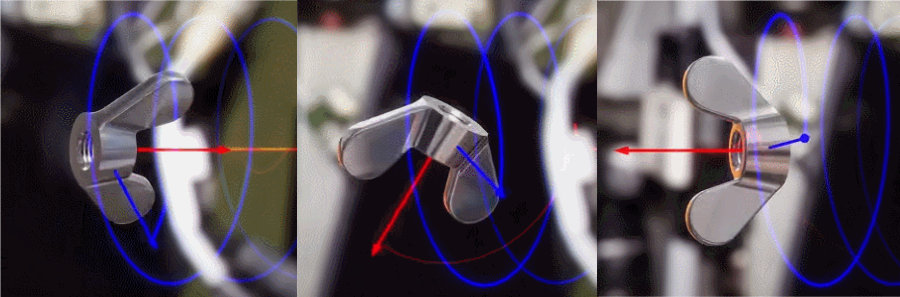
\includegraphics[width=0.9\textwidth]{dzhani.jpg}
\end{center}
   \caption{Một mô tả về hiệu ứng Dzhanibekov \cite{28}.}
\label{fig:10}
\end{figure*}

\begin{figure*}[t]
\begin{center}
% \fbox{\rule{0pt}{2in} \rule{.9\linewidth}{0pt}}
\includegraphics[width=1\textwidth]{layers.jpg}
\end{center}
   \caption{Minh họa các quá trình bên trong Trái Đất dẫn tới hiện tượng lật theo lý thuyết ECDO \cite{129}.}
\label{fig:11}
\end{figure*}

Nguyên lý đằng sau sự thay đổi nhanh chóng của trục quay Trái Đất nằm ở vật lý cơ học của các vật thể đang quay. Ví dụ điển hình của hiện tượng này là hiệu ứng Dzhanibekov, do nhà du hành vũ trụ người Nga Vladimir Dzhanibekov phát hiện \cite{37}, được minh họa trong Hình \ref{fig:10}. Một vật thể không quay hoàn hảo quanh một trong ba trục quán tính chính sẽ không duy trì được một trục quay cố định. Nếu nó quay gần trục chính thứ hai, nó sẽ trải qua những sự thay đổi đột ngột trong chuyển động quay. Mặc dù đây không hoàn toàn là điều mà chúng ta tin là xảy ra trong các lần lật nhanh của Trái Đất, nhưng điểm mấu chốt là khi không có tác động ngoại lực, chỉ có vật lý cơ học quay mới có thể giải thích sự thay đổi nhanh chóng của trục quay Trái Đất.

Cần lưu ý rằng Trái Đất gần như chắc chắn không trải qua hiệu ứng Dzhanibekov đơn giản và đồng đều. Nếu điều này xảy ra, chúng ta sẽ có thể phát hiện sự thay đổi dần dần trục quay của Trái Đất theo thời gian. Thay vào đó, chúng tôi tin rằng Trái Đất trải qua những gián đoạn định kỳ và đột ngột trong cấu trúc vật lý của nó, dẫn đến sự tách rời giữa "phần quay ở vỏ ngoài" (lớp vỏ/ lớp manti) và "phần quay bên trong" (lớp lõi). Nếu không có tác động bên ngoài, định luật bảo toàn động lượng góc xác định rằng Trái Đất không thể tự nhiên thay đổi trục quay một cách đột ngột, nên sự tách biệt giữa phần quay ở vỏ ngoài và phần quay bên trong là một trong những điều hiếm hoi, ngoại trừ va chạm từ bên ngoài lên Trái Đất, có thể gây ra hiện tượng lật nhanh chóng và đột ngột.

Quá trình cụ thể được cho là gây ra gián đoạn nội tại này trong Trái Đất là sự thay đổi trạng thái của cấu trúc sắt trong lõi Trái Đất (Hình \ref{fig:11}). Lớp lõi bên trong được cấu thành từ sắt ở dạng lục phương xếp chặt (Fe) \cite{141}. Khi hcp-Fe này chuyển sang trạng thái kim loại lỏng, nó giải phóng động năng và bị đẩy ra lớp lõi ngoài. Sự chuyển pha này làm giảm độ thẩm thấu từ của lõi, khiến từ trường Trái Đất suy yếu, đồng thời giải phóng nhiệt, hình thành các cấu trúc LLVP (vùng có vận tốc cắt thấp lớn) (Hình \ref{fig:12}) \cite{38} trong lớp manti và làm nóng bề mặt Trái Đất thông qua các đại dương sâu. Cả hai xu hướng này đều đã được ghi nhận rõ ràng trong vài thế kỷ gần đây và sẽ được bàn luận thêm trong bài viết này.


\begin{figure}[t]
\begin{center}
% \fbox{\rule{0pt}{2in} \rule{0.9\linewidth}{0pt}}
   \includegraphics[width=1\linewidth]{llvp.jpg}
\end{center}
   \caption{Hình ảnh chi tiết về LLVP bên dưới Nam Phi \cite{28}.}
\label{fig:12}
\label{fig:onecol}
\end{figure}


Cũng chính quá trình này bên trong Trái Đất, xảy ra theo chiều ngược lại, được cho là nguyên nhân thúc đẩy Trái Đất trở về trạng thái quay hiện tại của nó một cách khá nhanh chóng sau khi hiện tượng lật xảy ra.

\section{Bằng chứng về việc sắp xảy ra hiện tượng Trái Đất lật}

Có nhiều lý do để tin rằng chúng ta đang có nguy cơ sắp xảy ra lần lật Trái Đất tiếp theoc. Một thảm họa lớn chưa xảy ra trong nhiều thiên niên kỷ, đây là tần suất mà các sự kiện này dường như xảy ra, dựa trên các ghi chép lịch sử và dữ liệu. Dữ liệu mạnh mẽ nhất ủng hộ cho dự đoán sắp xảy ra lần lật Trái Đất tiếp theo là dữ liệu từ trường Trái Đất gần đây cho thấy từ trường Trái Đất đã suy yếu trong khoảng hai nghìn năm qua. Quá trình suy yếu này đang tăng tốc và đã đạt mức báo động trong vài thập kỷ gần đây.
Hình \ref{fig:14} minh họa từ trường Trái Đất vào năm 1590 và 2025 \cite{125,126}. Như thể hiện trong hình, từ trường đã suy yếu đáng kể.

Một chỉ số khác cho thấy từ trường Trái Đất suy yếu là vị trí của cực bắc từ trường Trái Đất (Hình \ref{fig:13}). Trước đây, cực bắc từ trường Trái Đất chủ yếu nằm ở Bắc Cực của Canada. Tuy nhiên, trong vài thế kỷ qua, nó đã di chuyển chậm và tăng tốc đáng kể trong vài thập kỷ gần đây. Hiện tại, nó đang di chuyển nhanh về phía nước Nga với tốc độ 55 km mỗi năm \cite{124}.

\begin{figure}[t]
\begin{center}
% \fbox{\rule{0pt}{2in} \rule{1\linewidth}{0pt}}
   \includegraphics[width=1\linewidth]{npw.jpg}
\end{center}
   \caption{Vị trí của cực bắc từ trường Trái Đất trong khoảng từ năm 1590 đến 2025, thể hiện theo từng mốc 5 năm \cite{142}.}
\label{fig:13}
\label{fig:onecol}
\end{figure}

\begin{figure*}[t]
\begin{center}
% \fbox{\rule{0pt}{2in} \rule{.9\linewidth}{0pt}}
\includegraphics[width=0.9\textwidth]{saa.jpg}
\end{center}
   \caption{Hình minh họa sự suy yếu của từ trường Trái Đất từ năm 1590 đến 2025. Dữ liệu được tính toán dựa trên các mô hình gufm1 và IGRF-14 \cite{125,126}.}
\label{fig:14}
\end{figure*}

\begin{figure}[t]
\begin{center}
% \fbox{\rule{0pt}{2in} \rule{1\linewidth}{0pt}}
   \includegraphics[width=1\linewidth]{ocean-highlight.jpg}
\end{center}
   \caption{Tốc độ ấm lên của đại dương có độ sâu lớn (sâu $>$2000 m) từ năm 1991 đến 2010, được khoanh tròn màu đỏ \cite{132}.}
\label{fig:15}
\label{fig:onecol}
\end{figure}

Từ trường của Trái Đất được cho là được tạo ra bởi một "dynamo bên trong" — tức là các cột dòng dung nham chuyển động vòng tròn trong lớp ngoài của lõi Trái Đất do ảnh hưởng của chuyển động quay \cite{123}. Sự suy yếu của từ trường là triệu chứng của các rối loạn sâu bên trong Trái Đất. Theo lý thuyết ECDO, những rối loạn này giải phóng nhiệt và cuối cùng dẫn đến sự tách rời giữa lớp manti và lớp lõi Trái Đất, gây ra hiện tượng Trái Đất lật \cite{1}.

Có rất nhiều dữ liệu xác nhận sự tồn tại của các quá trình tỏa nhiệt bên trong Trái Đất. Trái Đất ấm lên được ghi nhận qua nhiệt độ bề mặt đại lục và đại dương tăng dần \cite{127,128}, nồng độ CO2 khí quyển tăng cùng các luồng nhiệt của Trái Đất \cite{129,130} và sự suy giảm diện tích băng biển toàn cầu \cite{131}. Dữ liệu cho thấy mức CO2 và nhiệt độ tăng không phải là nguyên nhân của biến đổi khí hậu do con người mà là hệ quả sau cùng của lõi Trái Đất tỏa nhiệt \cite{129}.

Đáng chú ý nhất, các nghiên cứu về tốc độ ấm lên ở đại dương có độ sâu lớn (sâu $>$2000 mét) cho thấy không chỉ các đại dương sâu đang ấm lên mà tốc độ ấm mạnh nhất lại nằm ở tầng vực sâu (4000 - 6000 m). Sự ấm lên ở đáy đại dương này có trung tâm bên dưới 4000 mét \cite{132,129}, điều này sẽ không thể xảy ra nếu các đại dương được làm nóng từ phía trên bởi khí quyển. Những dữ liệu này cho thấy bằng chứng mạnh mẽ rằng các biến đổi khí hậu và từ trường gần đây được thúc đẩy bởi các quá trình diễn ra sâu bên trong Trái Đất. Hình \ref{fig:15} thể hiện tốc độ ấm lên toàn cầu của đại dương sâu từ năm 1991 đến 2010 \cite{132}.

\section{Mô hình hóa lần Trái Đất lật sắp tới}
\begin{figure}[b]
\begin{center}
% \fbox{\rule{0pt}{2in} \rule{1\linewidth}{0pt}}
   \includegraphics[width=1\linewidth]{saa-crop.jpeg}
\end{center}
   \caption{Một phép tính về điểm tới hạn dựa trên khu vực bất thường Nam Đại Tây Dương chỉ ra mốc thời gian là ngày 13 tháng 3, 2059 \cite{125,126}.}
\label{fig:16}
\label{fig:onecol}
\end{figure}

Dự đoán được thời điểm xảy ra lần lật tiếp theo của Trái Đất là một nhiệm vụ phức tạp. Hiện nay, mô hình tốt nhất mà chúng ta có được nằm ở từ trường Trái Đất - khu vực bất thường Nam Đại Tây Dương (SAA). Khu vực này ở phía trên Nam Đại Tây Dương có cường độ từ trường Trái Đất yếu nhất và được xác định là vùng có cường độ dưới 32.000 nanoTesla \cite{135}, mức yếu nhất kể từ năm 1590. Diện tích bề mặt mà khu vực bất thường Nam Đại Tây Dương chiếm trên Trái Đất đã tăng từ 1\% vào năm 1590 lên 21\% vào năm 2025 \cite{136}.

Để ước tính thời điểm Trái Đất có thể lật, tôi đã khớp dữ liệu về diện tích bề mặt của khu vực SAA với một phương trình điểm tới hạn theo hàm mũ - một mô hình hóa một hệ thống phức tạp khi đang tiến đến giai đoạn chuyển tiếp nghiêm trọng, trong đó hệ thống sẽ trải qua sự thay đổi đột ngột và mạnh mẽ. Các tính toán của tôi cho thấy thời điểm xảy ra lần lật Trái Đất tiếp theo sẽ là ngày 13 tháng 3 năm 2059 (Hình \ref{fig:16}). Dự đoán này sẽ càng chính xác hơn khi ta tiến gần đến điểm chuyển tiếp \cite{136}.

Các chỉ số khác như độ dao động của trục quay, các bất thường thời tiết, dữ liệu động đất và núi lửa cũng có thể giúp chúng ta có dự đoán tốt hơn về thời điểm khi nào có thể xảy ra lần Trái Đất lật tiếp theo.

\section{Dòng thời gian lịch sử ECDO}

Trong khi rất khó xác lập mốc thời gian chính xác cho các sự kiện ECDO trong quá khứ, có vẻ như đã có ít nhất 2 sự kiện ECDO trong thời kỳ Holocene. Hãy lưu ý tới ghi chép của Herodotus từ các tu sĩ Ai Cập rằng, \textit{"từ vị vua đầu tiên đến vị tư tế Hephaistos trị vì cuối cùng, đã có ba trăm bốn mươi mốt thế hệ con người... Trong thời gian này, họ nói rằng mặt trời đã bốn lần di chuyển khỏi vị trí mọc quen thuộc. Nơi mà bây giờ nó lặn thì trước đây nó đã từng mọc hai lần, và nơi mà bây giờ nó mọc thì trước đây nó đã từng lặn hai lần"} \cite{32}. Plato, sống vào thế kỷ thứ 5 TCN \cite{111}, nói rằng sau trận lụt đã nhấn chìm Atlantis chỉ trong một ngày một đêm vào 9.000 năm trước, \textit{"từ đó tới nay đã có nhiều trận đại hồng thủy, và những người sống sót ở các vùng núi không biết về chữ viết, trong suốt nhiều thế hệ chỉ tập trung vào việc mưu sinh"} \cite{112}, điều này cho thấy có thể đã xảy ra hơn hai lần Trái Đất lật kể từ cuối thời kỳ Younger Dryas vào khoảng năm 9700 TCN. Các bằng chứng vật lý được trình bày trong toàn bộ bài viết này và trong nghiên cứu của tôi \cite{2} cung cấp đầy đủ dữ liệu củng cố cho ghi chép của Plato.
Thời điểm ứng viên gần đây nhất cho một lần lật Trái Đất theo lý thuyết ECDO là trong giai đoạn từ năm 2300 đến 1600 TCN, gắn liền với nhiều ghi chép về các trận đại hồng thuỷ (Gun-Yu \cite{113,114,115}, Ogyges \cite{116,117}, Peru \cite{118,119}, Exodus \cite{120}), sự hủy diệt và bỏ hoang các nền văn minh (Mohenjo-Daro \cite{121}, Minoan Crete\cite{100,101}) và các hiện tượng vật lý bất thường (các sự kiện liên kết \cite{122}, sự kiện 4,2 nghìn năm \cite{90}) đã được xác định niên đại. Không có sự hội tụ bằng chứng đầy đủ nào gần đây hơn cho thấy có sự kiện thảm họa lớn.

\section{Kết luận}

Chiến dịch NANOOK là một nỗ lực trinh sát trong Chiến tranh Lạnh của Hoa Kỳ nhằm lập bản đồ Bắc Cực và bờ biển phía bắc Liên Xô sau Thế chiến II \cite{137}. Trong quá trình điều tra, họ phát hiện rằng cực từ nằm lệch về phía bắc từ 125 đến 200 dặm so với vị trí dự kiến dựa trên kết quả từ các chuyến thám hiểm trước đó. Theo đó, \textit{"Các nhà khoa học chính phủ đã dấy lên câu hỏi: Điều gì sẽ xảy ra khi cực từ và cực địa lý trùng nhau? Để trả lời câu hỏi này, dưới sự quản lý dự án của Tiến sĩ Paul A. Siple, Tập đoàn Rand đã được giao nhiệm vụ thực hiện các nghiên cứu trong phòng thí nghiệm, sử dụng các mô hình Trái Đất cấu tạo từ các hình cầu đồng tâm - một hình cầu bên trong đại diện cho lõi sắt nóng chảy mang điện từ của Trái Đất, với trục của nó xác định các cực 'từ'; và một hình cầu bên ngoài đại diện cho lớp vỏ Trái Đất quay quanh một trục cực 'địa lý'. Qua các thí nghiệm lặp đi lặp lại, người ta xác định rằng khi cực 'từ' tiến gần đến cực 'địa lý', cực 'từ' sẽ đến một điểm mà tại đó nó tăng tốc độ hội tụ như thể bị lực hướng tâm kéo về cực 'địa lý' và bất ngờ nhảy tới vị trí trùng nhau; nhưng thay vì trùng nhau, cực 'từ' sẽ nhanh chóng 'lật' quanh cực 'địa lý', rồi quay văng ra hướng xích đạo như thể bị lực ly tâm đẩy đi, và dừng lại ở một vị trí mà tại đó hai trục tạo thành một góc lệch xấp xỉ 89 độ. Sau khi quá trình 'lật cực' này xảy ra, các trục sẽ dần dần bắt đầu hội tụ trở lại trong thời gian dài"} \cite{138,139}.

Sau đó, \textit{"Tại một cuộc họp khoa học mà Thiếu tá White tham dự tại Lầu Năm Góc vào đầu năm 1948, các nhà khoa học đã thảo luận về việc có nên cảnh báo công chúng về hiện tượng lật cực sắp xảy ra hay không. Không ai trong số họ đồng ý giữ kín thông tin này với công chúng; tuy nhiên, họ cũng không thể thống nhất được cách thức công bố. Một số người lo ngại rằng chỉ riêng việc công chúng biết đến hiện tượng này cũng có thể phá vỡ nền tảng đạo đức của xã hội. Tuy nhiên, những lo ngại này dường như không có cơ sở, khi vào đầu những năm 1950, thông tin về hiện tượng lật cực đã được công bố trên một mục báo và một bài viết trên tạp chí, nhưng lại không nhận được bất kỳ phản hồi nào từ công chúng - những người dường như đã quá sững sờ, thiển cận hoặc hoài nghi để phản ứng"} \cite{138,139}.

Tại sao chúng ta lại không chú ý tới điều này? Có nhiều lý do để tin rằng Trái Đất đã từng lật. Bài viết này, cùng với phần hai, cung cấp bản tóm tắt súc tích về rất nhiều bằng chứng từ nhiều lĩnh vực cho thấy điều này đúng, chẳng hạn như các câu chuyện đại hồng thủy khắp thế giới, hóa thạch muối và sinh vật biển phủ khắp lục địa, các hầm trú ẩn cổ xưa dưới lòng đất, hài cốt động vật và cảnh quan địa chất thảm khốc. Con người được cho là xuất hiện từ hàng trăm nghìn năm trước, nhưng lịch sử hiện đại chỉ kéo dài vài nghìn năm. Liệu có thể là cứ sau một khoảng thời gian thì Trái Đất lại lật, các lục địa bị xóa sạch, và chúng ta buộc phải bắt đầu lại từ đầu — thời Đồ Đá — khiến những ghi chép về lịch sử cổ đại chỉ còn là vài câu chuyện thảm họa? Nếu vậy thì việc ngăn ngừa điều này tái diễn có thể là một trong những nhiệm vụ quan trọng nhất của nhân loại.

Để kết thúc, tôi xin để lại cho bạn ghi chép này trong Timaeus, được Plato viết lại, về một cuộc trò chuyện giữa Solon, một quốc vụ khanh người Athens, và các tư tế Ai Cập \cite{140}: \textit{"Một dịp, khi [Solon] muốn lôi kéo họ vào cuộc đối thoại về lịch sử cổ xưa, ông cố kể với họ truyền thuyết lâu đời nhất của chúng ta, về Phoroneus, được xem là người đầu tiên, và Niobe; ông tiếp tục kể về truyền thuyết Deucalion và Pyrrha sau Đại Hồng Thủy, cách họ sống sót và phả hệ của hậu duệ họ; và bằng cách kể về số năm của các sự kiện được nhắc tới, ông cố gắng tính toán các giai đoạn thời gian. Lúc đó một trong các tư tế, một cụ già bậc thầy, nói rằng: “Hỡi Solon, Solon, người Hy Lạp luôn là những đứa trẻ: Không có gì gọi là người Hy Lạp già.” Nghe vậy, ông hỏi, “Ngài muốn nói gì với câu đó?” Và vị tư tế đáp, “Tâm hồn các ngươi đều trẻ. Vì lẽ đó các ngươi không có niềm tin nào là cổ xưa và được truyền lại từ các truyền thống cũ, và cũng không có bất kỳ khoa học nào mang dấu vết của tuổi tác. Đó là lý do: Đã từng và sẽ còn xảy ra nhiều cuộc hủy diệt nhân loại, trong đó lớn nhất là do lửa và nước, và những cuộc hủy diệt nhỏ hơn bởi vô số hình thức khác. Thật vậy, câu chuyện được kể ở quốc gia các ngươi cũng như ở quốc gia chúng ta, rằng từng một lần Phaethon, con trai của Helios, điều khiển cỗ xe của cha mình, và vì không thể cầm lái đi đúng hướng nên đã đốt cháy mọi thứ trên mặt đất và bản thân thì chết bởi sét – câu chuyện đó, như được kể, mang dáng dấp truyền thuyết, nhưng sự thật nằm ở chỗ sự dịch chuyển của các thiên thể chuyển động quanh Trái Đất, và sự hủy diệt của những gì trên Trái Đất do ngọn lửa dữ, việc này lặp lại theo chu kỳ dài. Vào những thời điểm như vậy, tất cả những ai sống trên núi cao và vùng khô ráo sẽ chịu thiệt hại nhiều hơn những người sống gần sông hoặc biển; còn trường hợp của chúng ta, sông Nile cứu chúng ta bằng cách dâng nước lên cao — cũng như đã cứu chúng ta theo các cách khác. Và khi, ở những khoảng thời gian khác, các vị Thần thanh lọc mặt đất bằng lũ lụt, mọi mục đồng, người chăn thả trên núi được cứu, nhưng những người sống ở thành phố các ngươi thì bị dòng nước cuốn trôi xuống biển; còn ở đất nước chúng ta, không phải khi đó hay bất cứ lúc nào nước lại đổ từ trên xuống đồng ruộng, ngược lại nước thường dâng lên từ dưới lòng đất. Do đó, vì những lý do này, những gì được giữ lại ở đây được coi là cổ xưa nhất; sự thật là ở bất kỳ nơi nào không có quá nóng hoặc quá lạnh thì luôn tồn tại một giống người nào đó, khi nhiều, khi ít. Nếu có sự kiện nào cao quý hoặc vĩ đại hoặc nổi bật, dù xảy ra ở đất nước các người hay đất nước ta hoặc nơi khác mà chúng ta có biết, thì tất cả những sự kiện đó đều đã được ghi chép từ xa xưa và lưu giữ trong các đền thờ của chúng ta. Trong khi đó, người dân các ngươi và các dân tộc khác cứ mỗi lần, lại phải bắt đầu lại từ đầu với chữ viết và những nghệ thuật cần thiết cho một quốc gia văn minh. Rồi khi, sau một chu kỳ thời gian quen thuộc, như một tai họa lặp lại, trận hồng thủy từ trời lại đổ xuống quét sạch dân các ngươi, thì chẳng còn lại ai ngoài những người mù chữ và thiếu hiểu biết — khiến các ngươi lại trở nên như trẻ thơ, không còn ký ức gì về những gì đã xảy ra từ thuở xa xưa, dù là ở vùng đất này hay ở chính quê hương các ngươi. Chắc chắn rằng, những gia phả mà ngươi vừa kể, hỡi Solon, về người dân nước ngươi chẳng hơn gì những câu chuyện trẻ con. Thứ nhất, ngươi chỉ nhớ một trận đại hồng thủy, trong khi đã từng có nhiều trận đại hồng thủy đã xảy ra trước đó. Thứ hai, ngươi không hề hay biết rằng chính vùng đất nơi các ngươi đang sinh sống ngày nay từng là nơi sinh ra giống người cao quý và hoàn hảo nhất trong nhân loại. Chính từ họ mà các ngươi, cũng như toàn bộ thành bang hiện tại của ngươi, đã được sinh ra — từ một hạt mầm nhỏ còn sót lại một cách tình cờ. Nhưng điều này đã bị bỏ sót, vì suốt nhiều thế hệ, những người sống sót không có khả năng ghi chép lại bất kỳ điều gì. Thật vậy, hỡi Solon, đã từng có một thời — trước trận đại hồng thủy lớn nhất — quốc gia Athens ngày nay là lực lượng dũng cảm nhất trong chiến tranh và vô cùng xuất sắc trong mọi mặt tổ chức xã hội. Người ta nói rằng quốc gia đó sở hữu những tác phẩm nghệ thuật rực rỡ nhất và một thể chế chính trị cao quý nhất trong tất cả các quốc gia dưới bầu trời mà chúng ta từng được nghe kể lại”}.

Cũng những vị tư tế này, dĩ nhiên, còn kể cho Solon về nền văn minh cổ đại Atlantis: \textit{"Toàn bộ khu vực mà chúng ta đang nhắc đến ở đây, nằm trong cửa biển, rõ ràng chỉ là vịnh nhỏ có lối vào hẹp; còn phía bên kia mới thực sự là đại dương, và vùng đất bao quanh đại dương ấy mới đúng là lục địa thực sự theo đúng nghĩa đầy đủ và chân thực nhất. Trên hòn đảo Atlantis ấy, từng tồn tại một liên minh các vị vua có quyền lực lớn lao và kỳ diệu, kiểm soát toàn bộ hòn đảo, cũng như nhiều đảo khác và các phần của lục địa. Hơn thế nữa, trong khu vực bên trong Eo biển, họ đã cai trị vùng Libya cho đến tận Ai Cập, và châu Âu đến tận Tyrrhenia. Một lần nọ, liên minh hùng mạnh này đã tập hợp lại và tiến hành một cuộc tấn công nhằm khuất phục cả đất nước của các người lẫn đất nước của chúng ta, cũng như toàn bộ khu vực bên trong Eo biển. Chính thời điểm đó, hỡi Solon, lòng quả cảm và sức mạnh của người dân quốc gia các ngươi đã tỏa sáng trước toàn thế giới. Họ đã đứng lên như những chiến binh dũng cảm nhất, vượt trội trong nghệ thuật chiến tranh, vừa dẫn dắt người Hy Lạp, vừa chiến đấu đơn độc khi bị các đồng minh bỏ rơi. Sau khi đối mặt với những hiểm họa chết người, họ đã đánh bại quân xâm lược và dựng nên chiến tích hiển hách; nhờ vậy mà họ cứu được những người chưa bị nô dịch, và giải phóng tất cả chúng ta — những người sống trong khu vực thuộc về Heracles. Tuy nhiên, về sau đã xảy ra những trận động đất và lũ lụt kinh hoàng, và chỉ trong một ngày đêm tang thương, toàn bộ đội quân anh dũng ấy đã bị chôn vùi trong lòng đất, còn đảo Atlantis thì bị biển cả nhấn chìm và biến mất"}.

\section{Lời cảm ơn}

Cảm ơn The Ethical Skeptic, tác giả ban đầu của lý thuyết ECDO, đã hoàn thành luận án chuyên sâu, đột phá và chia sẻ nó với thế giới. Bộ luận thuyết gồm ba phần của ông \cite{1} vẫn là tài liệu nền tảng cho lý thuyết về ECDO (Hiệu ứng Dzhanibekov do quá trình tách rời tỏa nhiệt giữa lớp lõi và lớp manti của Trái Đất), và chứa đựng nhiều thông tin hơn so với phần trình bày ngắn gọn trong tài liệu này.

Cảm ơn Ankit đã xử lý dữ liệu tổng hợp các thảm họa trong Bảng 1.

Và dĩ nhiên, xin cảm ơn những người khổng lồ mà chúng ta đang đứng trên vai họ — những người đã thực hiện tất cả các nghiên cứu và điều tra giúp cho công trình này trở nên khả thi và đã nỗ lực mang lại ánh sáng cho nhân loại.

\clearpage
\twocolumn

\section{Hình ảnh bổ sung}


\begin{figure}[H]
\begin{center}
% \fbox{\rule{0pt}{2in} \rule{1\linewidth}{0pt}}
   \includegraphics[width=1\linewidth]{wave.jpg}
\end{center}
   \caption{Cận cảnh hiện tượng xói mòn dạng sóng parabol ở chân kim tự tháp Khafre \cite{27}.}
\label{fig:19}
\label{fig:onecol}
\end{figure}

\begin{figure}[H]
\begin{center}
% \fbox{\rule{0pt}{2in} \rule{1\linewidth}{0pt}}
   \includegraphics[width=1\linewidth]{star-stone.jpg}
\end{center}
   \caption{Bản đồ các vì sao được khắc lên đá trong một trong các trục hầm của kim tự tháp Khufu \cite{28}.}
\label{fig:20}
\label{fig:onecol}
\end{figure}

\begin{figure*}[t]
\begin{center}
% \fbox{\rule{0pt}{2in} \rule{.9\linewidth}{0pt}}
\includegraphics[width=1\textwidth]{deepsea.jpg}
\end{center}
   \caption{Hình ảnh minh họa hiện tượng nóng bất thường ở các tầng biển sâu và vực sâu, so sánh với đường cong làm ấm đại dương thông thường từ khí quyển. Dữ liệu nhiệt bất thường tổng thể lấy từ NOAA \cite{147}, dữ liệu phân bố nhiệt ở tầng sâu và vực sâu dựa trên nghiên cứu của Desbruyeres \cite{132}. Phần xử lý và trực quan hóa dữ liệu do The Ethical Skeptic thực hiện \cite{129}.}
\label{fig:21}
\end{figure*}

\begin{figure*}[t]
\begin{center}
% \fbox{\rule{0pt}{2in} \rule{.9\linewidth}{0pt}}
\includegraphics[width=1\textwidth]{sealevel.jpeg}
\end{center}
   \caption{Mực nước biển cho thấy mức độ dao động tăng 20\% trong vòng 75 năm tại 63 trạm quan trắc, cho thấy tốc độ dòng chảy đã tăng lên. Sự gia tăng mức độ dao động mực nước biển xảy ra đồng thời với các đợt xung nhiệt đại dương, cho thấy cả hai có thể đều do hiện tượng nóng lên từ sâu dưới đáy đại dương của Trái Đất \cite{2,129}.}
\label{fig:22}
\end{figure*}

\begin{figure*}[t]
\begin{center}
% \fbox{\rule{0pt}{2in} \rule{.9\linewidth}{0pt}}
\includegraphics[width=1\textwidth]{co2.jpg}
\end{center}
   \caption{Nồng độ CO2 trong khí quyển (ppm) đã tăng đều đặn trong 45 năm qua, có thể do nhiệt độ đại dương tăng lên. Nguồn: NOAA \cite{148,129}.}
\label{fig:23}
\end{figure*}

\begin{figure*}[t]
\begin{center}
% \fbox{\rule{0pt}{2in} \rule{.9\linewidth}{0pt}}
\includegraphics[width=1\textwidth]{ice.jpg}

\end{center}
   \caption{Diện tích băng biển toàn cầu đã giảm trong 45 năm qua, do Trái Đất ấm lên. Nguồn: ADS \cite{149}.}
\label{fig:24}
\end{figure*}

\clearpage
\twocolumn

{\small
\renewcommand{\refname}{Tài liệu tham khảo}
\bibliographystyle{ieee}
\bibliography{egbib}
}

\end{document}